\textbf{{1.层次结构概述}}

{下图总结了I/O软件的层次结构及每一层的主要功能。}

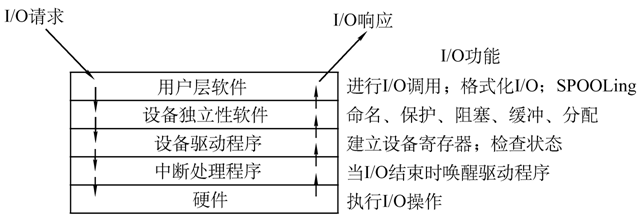
\includegraphics[width=2.29167in,height=0.78125in]{png-jpeg-pics/BA126AD149859BCD48B01C0444C33241.png}

\textbf{{2.中断处理程序}}

\textbf{a.
基本概念:}控制输入输出设备和内存与CPU之间的数据传送的主要方式。当完成I/O操作时,设备便向CPU发送一个中断信号,CPU响应中断后便转入中断处理程序。

\textbf{b. 中断过程:}① 唤醒被阻塞的驱动程序进程;②
保护被中断进程的CPU环境;③ 分析中断原因;④ 进行中断处理;⑤
恢复被中断进程的现场。

\textbf{{3.设备驱动程序}}

\textbf{a.
基本概念:}接受来自上层的设备独立性软件的抽象请求,将这些请求转换成设备控制器可以接受的具体命令,再将这些命令发送给设备控制器,并监督这些命令正确执行。\textbf{设备驱动程序是操作系统中唯一知道设备控制器中设置了多少个寄存器以及这些寄存器有何用途的程序}。

{\textbf{b. 设备驱动程序的处理过程:}}① 将抽象要求转换为具体要求;②
检查I/O请求的合法性;③ 读出和检查设备的状态;④ 传送必要参数;⑤
设置工作方式;⑥ 启动I/O设备。

\textbf{{4.设备独立性软件}}

\textbf{a.
基本概念:}实现一般设备都需要的I/O功能,并向用户空间软件提供一个统一的接口。设备独立性软件通常应实现的功能包括设备驱动程序的统一接口,设备命名,设备保护,提供与设备无关的逻辑块,缓冲、存储设备的块分配,独占设备的分配和释放,出错处理。

\textbf{{5.用户层软件}}

一般来说,大部分I/O软件都包含在操作系统中,但是仍有一部分是\textbf{由与用户程序链接在一起的库函数,甚至运行于内核之外的程序构成的}。通常的系统调用包括I/O系统调用,是由库函数实现的。SPOOLing系统也处于这一层上。
